\documentclass[a4paper,11pt]{article}
\usepackage[T1]{fontenc}
\usepackage[utf8]{inputenc}
\usepackage{lmodern}
\usepackage[top=2cm,left=2.5cm,right=2.5cm,bottom=2cm]{geometry} % Géométrie de la page, modifier selon le besoin
\usepackage{graphicx}
\usepackage{subcaption}

\title{}
\author{}
\date{}


\begin{document}

\maketitle
\section{Parameters}


\section{Fiber 5}
\begin{itemize}
    \item 4th April 2016
    \item In air
    \item $\lambda = 808nm$
    \item 51$\times$51 dots scans
\end{itemize}

\begin{figure}[htb]
  \begin{subfigure}[b]{.20\linewidth}
    \centering
    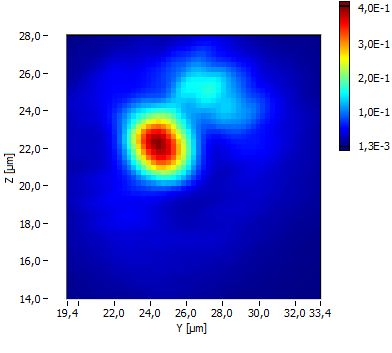
\includegraphics[width=\textwidth]{Fibre5/scan_021_g1.jpg}
    \caption{$d=1.8\mu m$}
  \end{subfigure}
  \begin{subfigure}[b]{.20\linewidth}
    \centering
    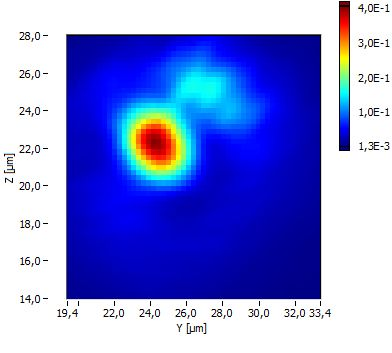
\includegraphics[width=\textwidth]{Fibre5/scan_022_g1.jpg}
    \caption{$d=2.8\mu m$}
  \end{subfigure}
  \begin{subfigure}[b]{.20\linewidth}
    \centering
    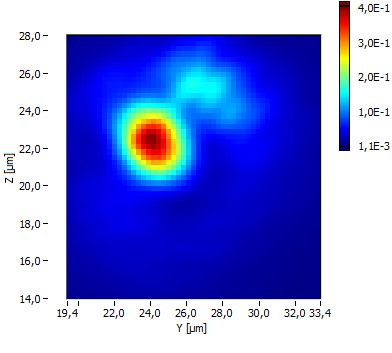
\includegraphics[width=\textwidth]{Fibre5/scan_023_g1.jpg}
    \caption{$d=3.8\mu m$}
  \end{subfigure}
  \begin{subfigure}[b]{.20\linewidth}
    \centering
    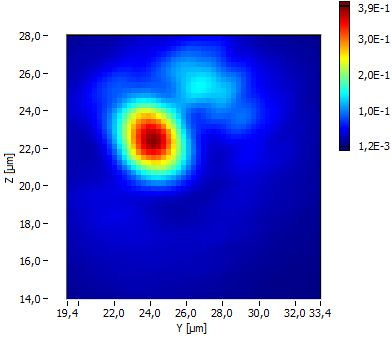
\includegraphics[width=\textwidth]{Fibre5/scan_024_g1.jpg}
    \caption{$d=6.8\mu m$}
  \end{subfigure}
  \begin{subfigure}[b]{.20\linewidth}
    \centering
    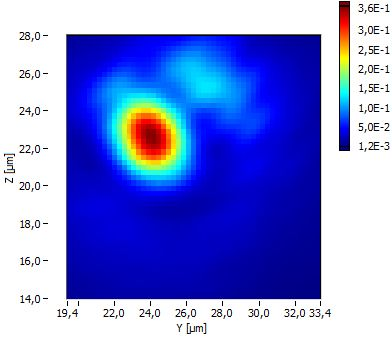
\includegraphics[width=\textwidth]{Fibre5/scan_025_g1.jpg}
    \caption{$d=9.8\mu m$}
  \end{subfigure}
  \begin{subfigure}[b]{.20\linewidth}
    \centering
    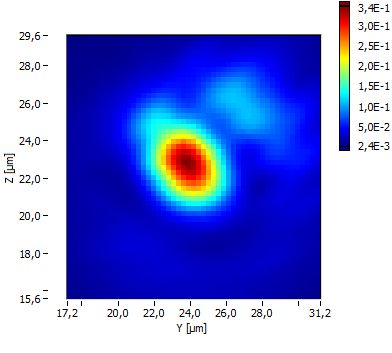
\includegraphics[width=\textwidth]{Fibre5/scan_026_g1.jpg}
    \caption{$d=12.8\mu m$}
  \end{subfigure}
  \begin{subfigure}[b]{.20\linewidth}
    \centering
    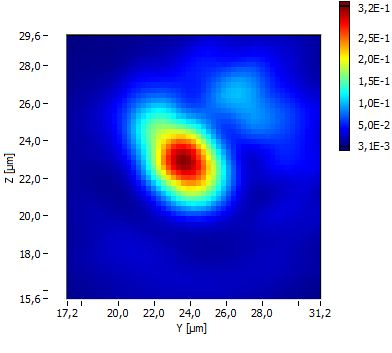
\includegraphics[width=\textwidth]{Fibre5/scan_027_g1.jpg}
    \caption{$d=16.8\mu m$}
  \end{subfigure}
  \begin{subfigure}[b]{.20\linewidth}
    \centering
    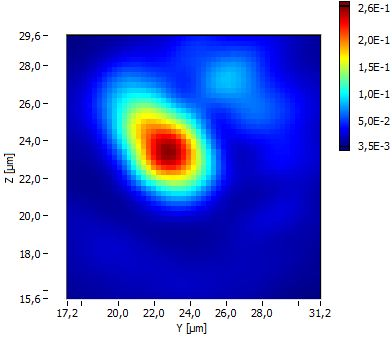
\includegraphics[width=\textwidth]{Fibre5/scan_028_g1.jpg}
    \caption{$d=21.8\mu m$}
  \end{subfigure}
  \begin{subfigure}[b]{.20\linewidth}
    \centering
    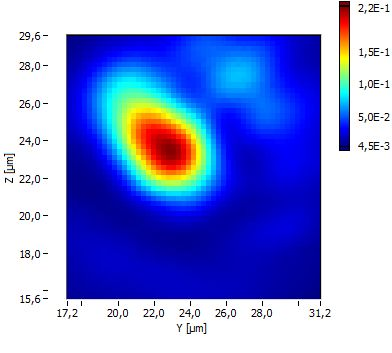
\includegraphics[width=\textwidth]{Fibre5/scan_029_g1.jpg}
    \caption{$d=26.8\mu m$}
  \end{subfigure}
  \begin{subfigure}[b]{.20\linewidth}
    \centering
    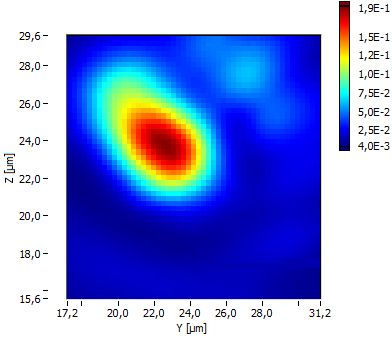
\includegraphics[width=\textwidth]{Fibre5/scan_030_g1.jpg}
    \caption{$d=31.8\mu m$}
  \end{subfigure}
  \begin{subfigure}[b]{.20\linewidth}
    \centering
    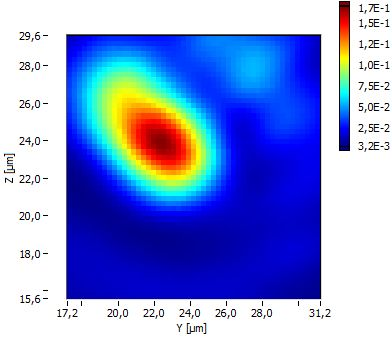
\includegraphics[width=\textwidth]{Fibre5/scan_031_g1.jpg}
    \caption{$d=36.8\mu m$}
  \end{subfigure}
  \begin{subfigure}[b]{.20\linewidth}
    \centering
    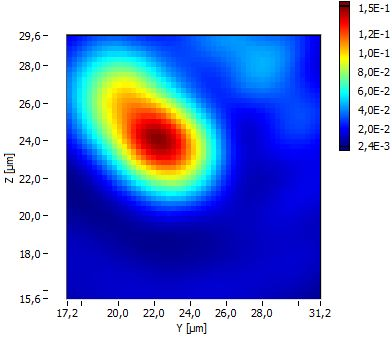
\includegraphics[width=\textwidth]{Fibre5/scan_032_g1.jpg}
    \caption{$d=41.8\mu m$}
  \end{subfigure}
  \begin{subfigure}[b]{.20\linewidth}
    \centering
    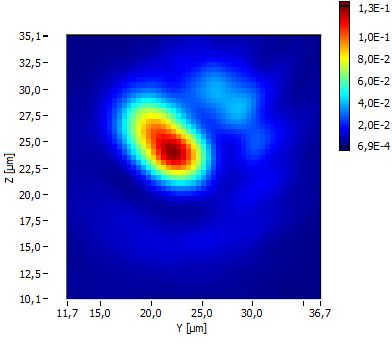
\includegraphics[width=\textwidth]{Fibre5/scan_033_g1.jpg}
    \caption{$d=46.8\mu m$}
  \end{subfigure}
  \hspace{8mm}
  \begin{subfigure}[b]{.20\linewidth}
    \centering
    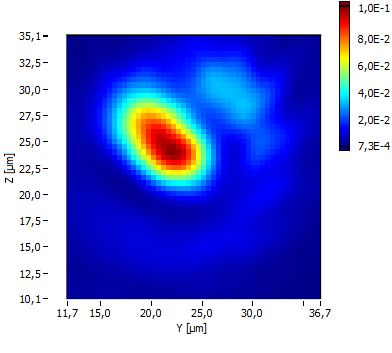
\includegraphics[width=\textwidth]{Fibre5/scan_034_g1.jpg}
    \caption{$d=51.8\mu m$}
  \end{subfigure}
\end{figure}

\newpage
\section{Fiber 6}
\begin{itemize}
    \item 7th April 2016
    \item In air
    \item $\lambda = 808nm$
    \item 31$\times$31 dots scans
\end{itemize}
\begin{figure}[htb]
  \begin{subfigure}[b]{.19\linewidth}
    \centering
    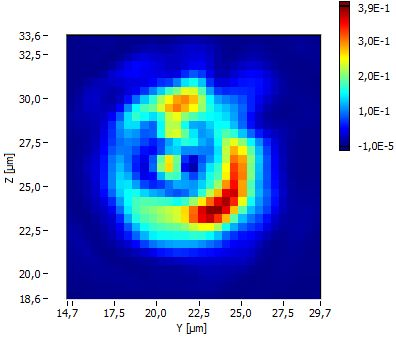
\includegraphics[width=\textwidth]{Fibre6/scan_006_g1.jpg}
    \caption{$d=4\mu m$}
  \end{subfigure}
  \begin{subfigure}[b]{.19\linewidth}
    \centering
    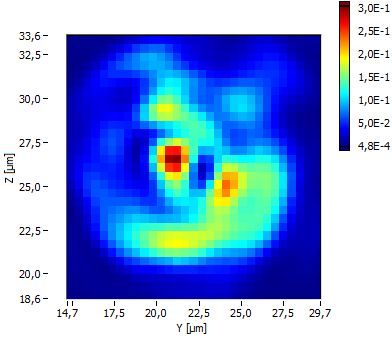
\includegraphics[width=\textwidth]{Fibre6/scan_007_g1.jpg}
    \caption{$d=14\mu m$}
  \end{subfigure}
  \begin{subfigure}[b]{.19\linewidth}
    \centering
    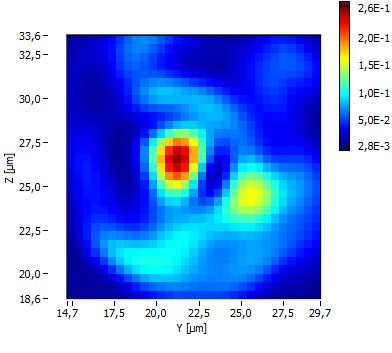
\includegraphics[width=\textwidth]{Fibre6/scan_008_g1.jpg}
    \caption{$d=24\mu m$}
  \end{subfigure}
  \begin{subfigure}[b]{.19\linewidth}
    \centering
    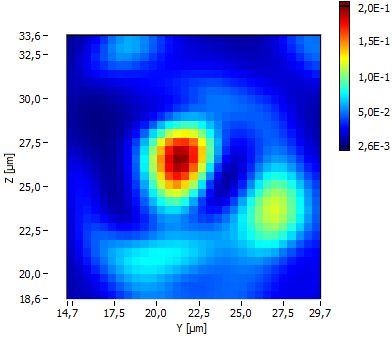
\includegraphics[width=\textwidth]{Fibre6/scan_009_g1.jpg}
    \caption{$d=34\mu m$}
  \end{subfigure}
  \begin{subfigure}[b]{.19\linewidth}
    \centering
    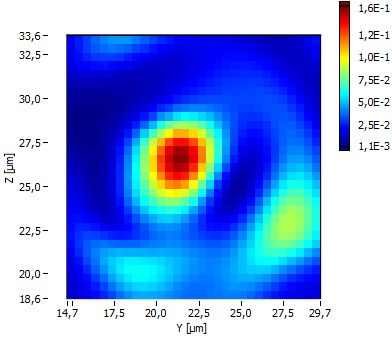
\includegraphics[width=\textwidth]{Fibre6/scan_010_g1.jpg}
    \caption{$d=44\mu m$}
  \end{subfigure}
  \begin{subfigure}[b]{.19\linewidth}
    \centering
    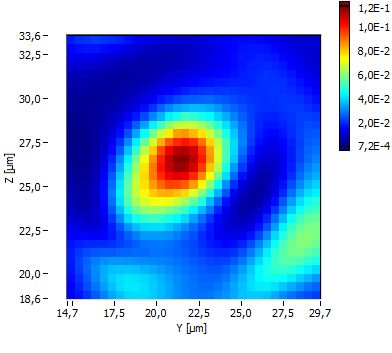
\includegraphics[width=\textwidth]{Fibre6/scan_011_g1.jpg}
    \caption{$d=54\mu m$}
  \end{subfigure}
  \begin{subfigure}[b]{.19\linewidth}
    \centering
    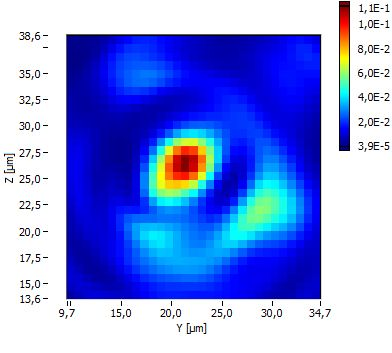
\includegraphics[width=\textwidth]{Fibre6/scan_012_g1.jpg}
    \caption{$d=54\mu m$}
  \end{subfigure}
\end{figure}

\end{document}
